\chapter{Protocolli Automotive} %\label{1cap:spinta_laterale}
% [titolo ridotto se non ci dovesse stare] {titolo completo}
%

\begin{citazione}
In questo capitolo verranno illustrati i dettagli sui principali protocolli utilizzati nel mondo \emph{Automotive}, evidenziando punti di forza e debolezze. Successivamente, verrà effettuato un confronto tra questi in termini di prestazioni, applicabilità, costi, ecc.
\end{citazione}

\section{CAN}

\subsection{Caratteristiche del protocollo}
Il protocollo \emph{CAN} (Controller Area Network) è un protocollo basato su scambio di messaggi che permette a più dispositivi di trasmettere informazioni in maniera affidabile e in logica basata su \textbf{priorità}. Tutti i messaggi (o "\emph{frame}") inviati sono ricevuti da tutti i dispositivi connessi alla rete e, per questa ragione, la tipica topologia di rete usata in sinergia con \emph{CAN} è \textbf{BUS}, ovvero tutti i dispositivi appartenenti alla rete vengono collegati su un singolo cavo detto anche \emph{backbone}. Inoltre, è un protocollo \textbf{multi-master} \cite{huang_2019_invehicle}, in quanto non ha bisogno di un nodo master che fa da arbitro per l'intera rete ma tutti i nodi connessi sono in grado di comunicare autogestendosi, utilizzando come schema di arbitraggio \textbf{CSMA/CD} (Carrier-Sense Multiple Access with Collision Detection) \cite{can_notes}. Con questo schema, un dispositivo che vuole trasmettere un messaggio si mette prima in ascolto sul cavo e, se non rileva trasmissioni in corso, comincia a trasmettere il messaggio ascoltando quello che sta inviando. Se nel mentre che sta inviando il messaggio rileva un'interferenza, generata dall'arrivo di un altro messaggio già in fase di trasmissione, ferma immediatamente la trasmissione, trasmette una sequenza di \textbf{jamming} con lo scopo di avvertire gli altri dispositivi che è avvenuta una collisione e attende un tempo casuale prima di ritrasmettere (ovviamente dopo aver stabilito che il canale è libero) \cite{wikipedia_csmacd}. Uno schema per comprendere meglio il funzionamento dell'algoritmo \textbf{CSMA/CD} è mostrato nella \autoref{fig:csmacd-scheme}.
\begin{figure}[h]
    \centering
    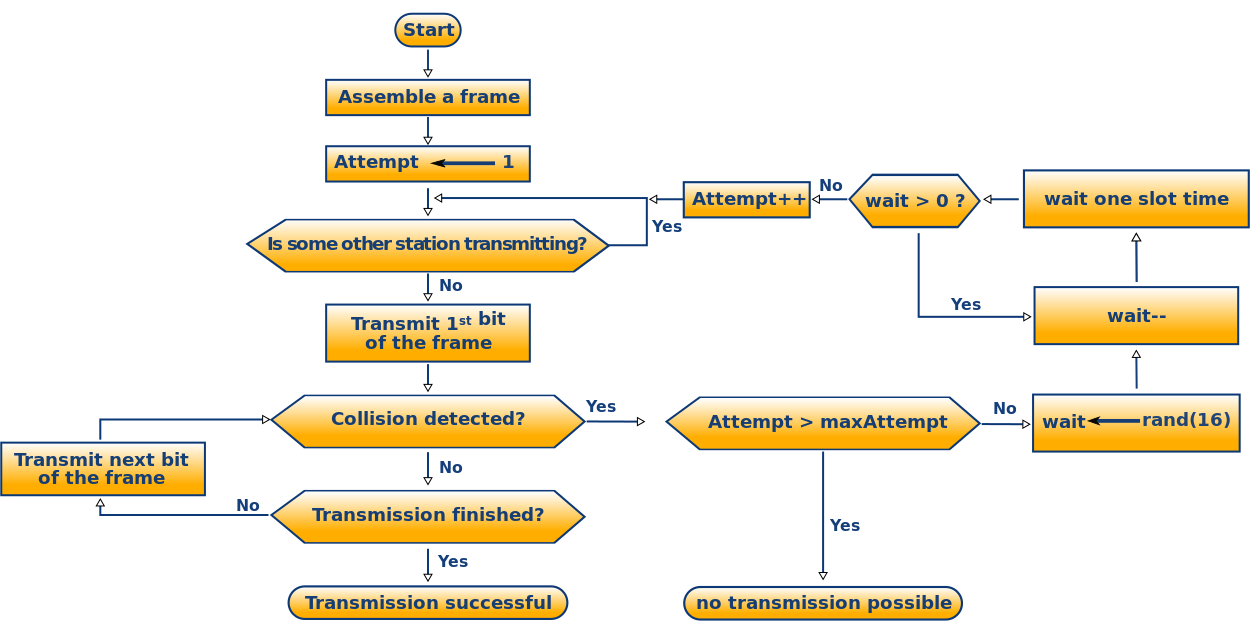
\includegraphics[width=0.7\textwidth]{capitoli/figure-protocolli/CSMACD-Algorithm.png}
    \caption{Diagramma di flusso di un algoritmo \textbf{CSMA/CD} con ritrasmissione}
    \label{fig:csmacd-scheme}
\end{figure}

Ogni dispositivo connesso alla rete viene chiamato \textbf{nodo} e deve essere composto almeno da una \emph{CPU} (processore per far funzionare tutto il dispositivo), un controller \emph{CAN} (componente che sappia parlare il protocollo \emph{CAN}) e un \emph{ricetrasmettitore} (componente che "legge e scrive" sui cavi elettrici).\\
È il protocollo più utilizzato in ambito \emph{Automotive} in quanto il suo utilizzo ha i seguenti vantaggi:

\begin{itemize}
    \item È un protocollo che richiede un cablaggio semplicissimo e poco costoso (un semplice cavo con due fili), riducendo la latenza, il peso della rete (in termini di kilogrammi), il numero di cavi necessari e il numero di errori;
    \item È completamente centralizzato e, per questa ragione, basta un qualunque punto di aggancio alla rete per accedere a tutto il traffico in circolazione e comunicare con tutte le \emph{ECU} connesse. Questo semplifica di molto il logging delle informazioni per fini diagnostici e la configurazione delle centraline;
    \item È molto robusto contro interferenze elettromagnetiche e disturbi elettrici, rendendolo ideale per applicazioni \textbf{safety-critical};
    \item Grazie all'integrazione di una logica basata su \textbf{priorità}, messaggi con \emph{ID} associati ad una priorità alta sono i primi ad accedere alla rete, senza causare interruzioni agli altri messaggi;
    \item Eliminando kilometri di cavi elettrici in eccesso, permette di ridurre il peso totale dell'automobile su cui è installata la rete migliorando anche i consumi di carburante;
    \item Dal momento che i chip e la strumentazione necessaria è molto semplice ed economica, abbassando di molto il costo necessario alla creazione della rete e delle \emph{ECU};
    \item Prevede meccanismi di correzione e rilevazione degli errori molto efficaci, permettendo alle informazioni di arrivare integre a destinazione;
    \item È facile aggiungere o rimuovere nodi dalla rete. \cite{can_bus_dewesoft}
\end{itemize}

\begin{figure}[h]
    \begin{subfigure}{0.45\textwidth}
        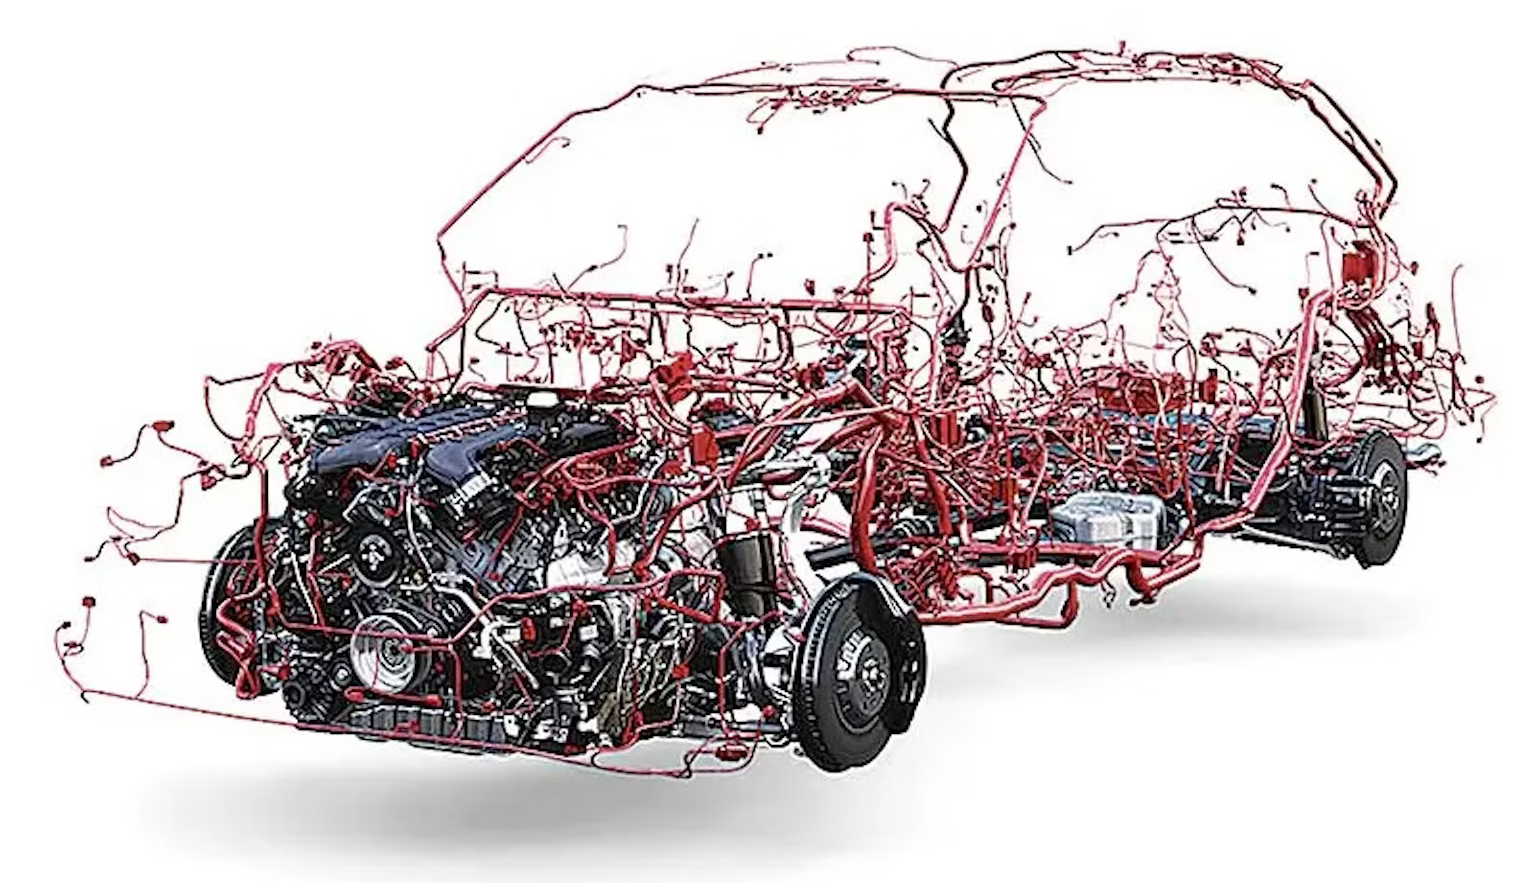
\includegraphics[width=1\textwidth]{capitoli/figure-protocolli/electrical-wiring-no-can.png}
        \caption{Cablaggio tipico di un'automobile che \textbf{NON} utilizza \emph{CAN}}
        \label{fig:electrical-wiring-no-can}
    \end{subfigure}
    \hfill
    \begin{subfigure}{0.45\textwidth}
        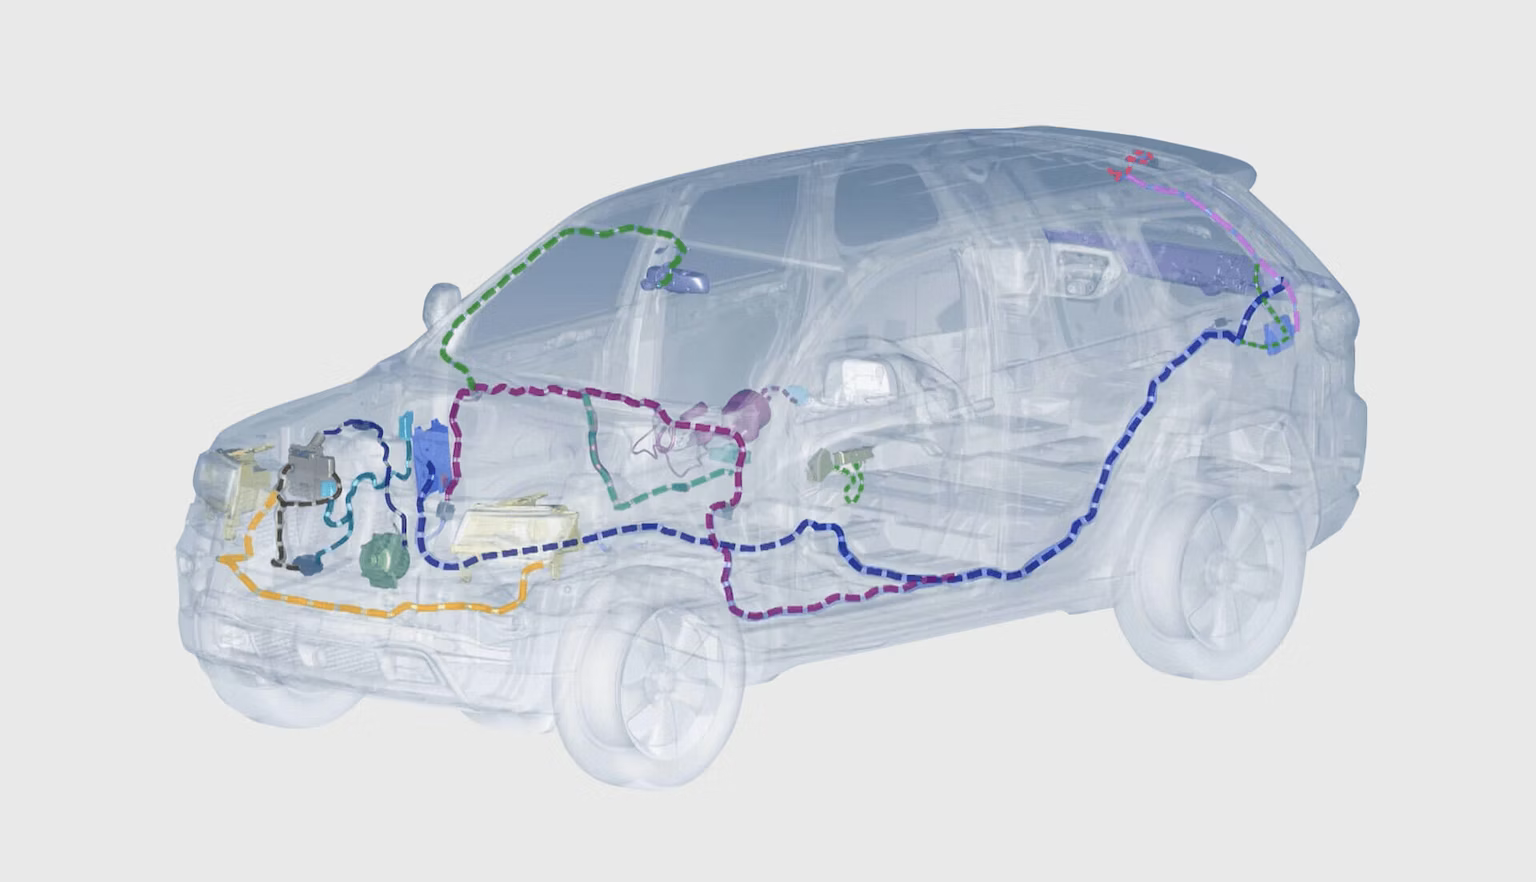
\includegraphics[width=1\textwidth]{capitoli/figure-protocolli/electrical-wiring-can.png}
        \caption{Cablaggio tipico di un'automobile che utilizza \emph{CAN}}
        \label{fig:electrical-wiring-can}
    \end{subfigure}
    \caption{Differenza di cablaggi con e senza \emph{CAN}}
    \label{fig:electrical-wiring-differences}
\end{figure}

Per via dei motivi sopracitati, oltre ad essere il protocollo più utilizzato in campo \emph{Automotive} è anche utilizzato in moltissimi altri ambiti, tra cui:

\begin{itemize}
    \item Aeronautica;
    \item Ascensori ed elevatori;
    \item Industrie e fabbriche;
    \item Navi;
    \item Elettrodomestici casalinghi come lavatrici, asciugatrici, ecc. \cite{can_bus_dewesoft}
\end{itemize}

\subsection{Struttura dei messaggi}
Ogni messaggio \emph{CAN} ha una struttura ben definita ed è composto da \textbf{header}, \textbf{payload} e \textbf{trailer}. Inoltre, è possibile individuare due tipologie di messaggi che sono \textbf{standard} e \textbf{esteso}, la cui unica vera differenza sta nella presenza di un campo \emph{ID} aggiuntivo nel messaggio (quindi cambia solo la lunghezza complessiva del messaggio).

\begin{figure}[h]
    \centering
    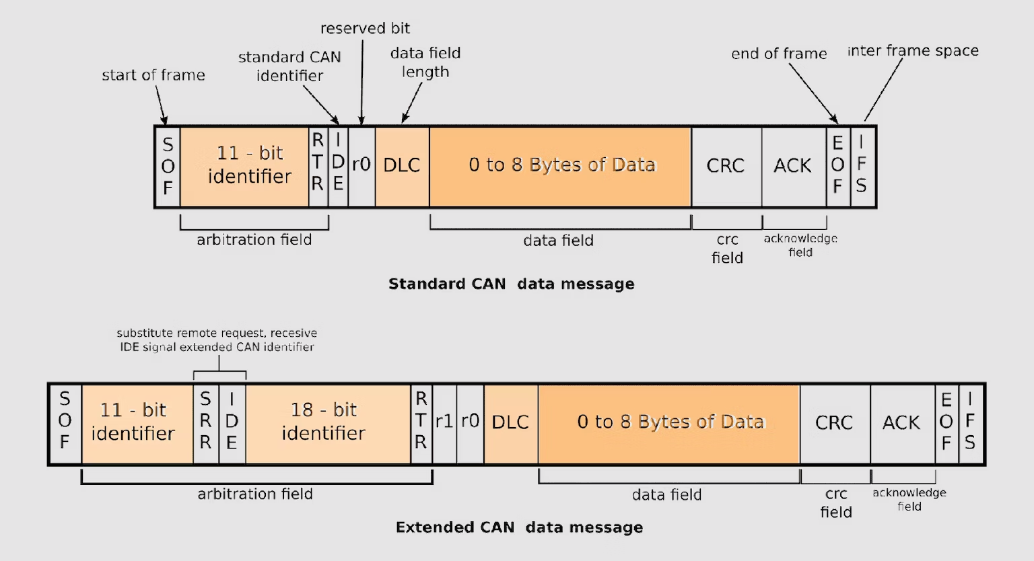
\includegraphics[width=0.7\textwidth]{capitoli/figure-protocolli/can-data-message-structure.png}
    \caption{Struttura dei messaggi \emph{CAN} \textbf{standard} ed \textbf{estesi}}
    \label{fig:can-message-structure}
\end{figure}

I vari campi di un tipico messaggio \emph{CAN} \textbf{standard} sono:
\begin{itemize}
    \item \textbf{SOF} (Start of Frame): 1 bit che indica l'inizio del messaggio e sincronizza i nodi dopo un periodo di inattività;
    \item \textbf{ID}: 11 bit che definiscono la priorità del messaggio, dove un identificativo più basso corrisponde ad una priorità più alta;
    \item \textbf{RTR}: 1 bit che viene impostato a $0$ (o \emph{dominante}) quando quello che si sta inviando è una \textbf{richiesta di informazione} (non un'informazione) e $1$ (o \emph{recessivo}) in caso contrario. Quando il bit viene impostato a $0$, non viene inviato nessun dato e l'\textbf{ID} determina l'informazione richiesta (quindi il nodo \emph{target});
    \item \textbf{IDE} (Identifier Extension): 1 bit che determina se il pacchetto è standard ($0$) o esteso ($1$);
    \item \textbf{r0}: 1 bit riservato che è privo di significato e lasciato per eventuali sviluppi futuri. Di solito è lasciato a $0$, ma anche se impostato a $1$ non fa differenza e viene accettato lo stesso;
    \item \textbf{DLC} (Data Length Code): 4 bit che indicano la lunghezza in \textbf{byte} del payload che contiene il messaggio;
    \item \textbf{Data}: 64 bit che indicano il dato che si sta inviando con il messaggio;
    \item \textbf{CRC} (Cyclic Redundancy Check): 16 bit che indicano il \textbf{checksum}, ovvero una \emph{somma} associata al campo \textbf{data} che viene utlizzata, tramite particolari operazioni matematiche, per effettuare rilevamento degli errori;
    \item \textbf{ACK} (ACKnowledgment): 1 bit che determina se un messaggio è stato ricevuto con successo ($0$) oppure sono stati rilevati degli errori ($1$). Chi invia il messaggio imposta il bit a $1$, metre chi riceve con successo imposta il bit a $0$;
    \item \textbf{EOF} (End of Frame): 7 bit che denotano la fine di un messaggio \emph{CAN}.
    \item \textbf{IFS} (Inter Frame Space): 3 bit recessivi (impostati a $1$) che separano il messaggio appena trasmesso da un nuovo messaggio. Dopo i primi 3 bit a $1$, il primo bit dominante (impostato a $0$) rilevato corrisponderà ad un bit \textbf{SOF}. \cite{can_bus_dewesoft} \cite{wikipedia_canbus}
\end{itemize}

Oltre ai campi di un messaggio \emph{standard}, i campi aggiuntivi in un messaggio \textbf{esteso} sono i seguenti:
\begin{itemize}
    \item \textbf{SRR} (Substitute Remote Request): 1 bit impostato a $1$ che serve a far prevalere sempre i messaggi \emph{standard} durante l'arbitraggio;
    \item \textbf{ID}: 18 bit che si aggiungono al primo campo \textbf{ID}, componendo un identificativo di 29 bit totali;
    \item \textbf{R1}: 1 bit riservato come \textbf{R0}, quindi anche in questo caso il valore associato a questo campo non ha significato e viene accettato qualunque sia.
\end{itemize}

Un'altra piccola differenza è che il campo \textbf{IDE} è posizionato prima del bit \textbf{RTR} e, in mezzo a questi due campi è posizionato il secondo campo \textbf{ID}.

\subsection{\emph{Bit stuffing}}
Per inviare i dati, a livello fisico, \emph{CAN} utilizza una codifica chiamata \textbf{NRZ} (Non-Return-to-Zero), ovvero il bit $1$ è codificato con un un voltaggio \emph{alto} mentre il bit $0$ con un voltaggio \emph{basso} e per codificare $n$ bit consecutivi basta inviare $n$ segnali \emph{alti} o \emph{bassi} in base al bit che si vuole inviare. Inoltre, la codifica può essere utilizzata secondo due tipologie:
\begin{itemize}
    \item \textbf{Unipolare}: il segnale \emph{alto} (quindi il bit $1$) è identificato da una differenza di voltaggio \textbf{positiva} (detto anche \emph{bias}), mentre il segnale \emph{basso} è identificato dall'assenza di un \emph{bias};
    \item \textbf{Bipolare}: il bit $1$ è codificato da un \emph{bias} positivo mentre il bit $0$ da un \emph{bias} negativo.
\end{itemize}

Esiste anche una codifica che fa da controparte, chiamata \textbf{RZ} (Return-to-Zero), nella quale un bit è identificato da una variazione di voltaggio seguito dal ritorno al valore \emph{normale} (nel caso dell'unipolare, il bit $0$ è identificato semplicemente dall'assenza di \emph{bias}). Una differenza tra le due codifiche (in versione unipolare) è mostrata in \autoref{fig:nrz-vs-rz}.
\begin{figure}[h]
    \centering
    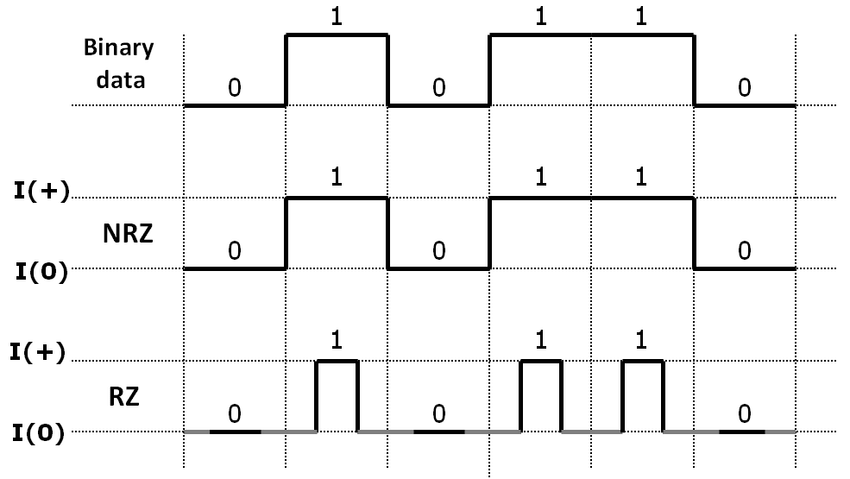
\includegraphics[width=0.5\textwidth]{capitoli/figure-protocolli/nrz-vs-rz.png}
    \caption{Differenza tra codifica \textbf{NRZ} e \textbf{RZ}, entrambe unipolari}
    \label{fig:nrz-vs-rz}
\end{figure}

Osservando le due codifiche, per inviare due bit $1$ con \textbf{NRZ} basta inviare due impulsi consecutivi alti, mentre con \textbf{RZ} bisogna inviare un impulso \emph{alto} seguito da un'assenza di \emph{bias} e, di nuovo un impulso \emph{alto} seguito da un'assenza di \emph{bias}. \cite{wikipedia_nrz}\\
Per via della natura della codifica \textbf{NRZ}, durante l'invio di molti bit consecutivi uguali c'è il rischio che i nodi perdano la sincronia e non siano più in grado di distinguere correttamente i bit inviati, questo poichè la polarità non varia per lunghi periodi di tempo. A questo proposito, l'invio dei messaggi con questa codifica viene affiancato da una tecnica chiamata \textbf{bit stuffing}, ovvero dopo l'invio di una certa soglia di bit uguali consecutivi viene inviato un bit di polarità inversa che non ha significato nel messaggio ma serve solo a mantenere i nodi sincronizzati (il bit viene detto \emph{di stuffing}). Ad esempio, immaginando che la soglia di bit consecutivi sia 4, se un nodo deve inviare la sequenza $111111$ (sei bit $1$ consecutivi), invierà la sequenza $1111011$ (dopo 4 bit invierà un bit \emph{di stuffing}). Ovviamente, il nodo che riceve il messaggio è a conoscenza della tecnica, è in grado di rimuovere correttamente i bit \emph{di stuffing} senza compromettere l'integrità del messaggio e nel momento in cui riceve un numero di bit consecutivi uguali al di sopra della soglia prestabilita rileva una violazione della codifica (nel caso di \emph{CAN} dopo ogni 5 bit uguali consecutivi, \textbf{DEVE} essere inviato un bit \emph{di stuffing}).

\subsection{Tipologie di messaggi}
Il protocollo \emph{CAN} prevede quattro tipologie di messaggi (o \emph{frame}), che si distinguono in base al compito che devono svolgere.
\subsubsection{Data Frames}
Questa tipologia di frame è l'unica che prevede l'utilizzo del campo \textbf{Data} e un \textbf{DLC} diverso da 0. È, quindi, la tipologia di messaggio che un nodo invia per condividere informazioni con uno o più nodi, associando all'identificativo il tipo di dato inviato e la priorità.

\subsubsection{Remote Frames}
Questa tipologia di frame permette ad un nodo di richiedere una specifica informazione, identificata dal campo \textbf{ID}. Anche se di solito le \emph{ECU} inviano le informazioni sulla rete di propria iniziativa quando l'informazione è pronta, a volte un nodo destinazione può richiedere uno specifico dato da uno specifico nodo. Questa tipologia di messaggio ha un payload vuoto in quanto non vuole inviare informazioni ma, tuttavia, il campo \textbf{DLC} è diverso da zero ed indica la lunghezza del dato \textbf{richiesto} e non "\textbf{inviato}". Infine, il campo \textbf{RTR} in questo caso è posto a $1$ (a differenza dei \emph{data frame}) in modo da associare una priorità più bassa a questa tipologia di messaggio e fargli perdere l'arbitraggio in caso di contesa con un \emph{data frame}. \cite{wikipedia_canbus}.

\subsubsection{Error Frames}
Questa tipologia di frame permette ai nodi, come espone in maniera molto chiara il nome, di segnalare eventuali errori rilevati a tutta la rete. La struttura di questi frame non segue quella descritta in precedenza ma è composta solo da 2 parti:
\begin{itemize}
    \item \textbf{Error flags}: tra 6 e 12 bit tutti \emph{dominanti} o tutti \emph{recessivi}, ottenuti dalla sovrapposizione di \emph{error frame} generati da nodi diversi;
    \item \textbf{Error Delimiter}: 8 bit tutti \emph{recessivi} che delimitano il frame.
\end{itemize}

La caratteristica fondamentale che contraddistingue questa tipologia di frame è il fatto che il campo \textbf{Error flags} è composto da bit uguali e non presenta bit \emph{di stuffing}, realizzando una violazione della regola del \emph{bit stuffing}.
Inoltre, ci sono due tipolgie di questi frame:
\begin{itemize}
    \item \textbf{Attivo}: tutti i bit del campo \textbf{Error flags} sono \emph{dominanti} e questo tipo di frame è generato da un nodo in modalità \textbf{attiva}, ovvero un nodo che per primo ha rilevato un errore;
    \item \textbf{Passivo}: tutti i bit del campo \textbf{Error flags} sono \emph{recessivi} e questo tipo di frame è generato da un nodo che è passato dallo stato \textbf{attivo} allo stato \textbf{passivo}.
\end{itemize}

Come già accennato, la tipologia di frame generato dipende dalla modalità in cui si trova il nodo, che può essere:
\begin{itemize}
    \item \textbf{Attiva}: modalità di default di ogni nodo. In questa modalità il nodo è in grado di inviare dati e frame di errore \textbf{attivi};
    \item \textbf{Passiva}: modalità in cui entrano i nodi che hanno generato un determinato numero di errori. In questa modalità i nodi sono in grado di inviare frame di errore \textbf{passivi} e sono in grado di inviare anche dati, tuttavia con l'obbligo di attendere 8 bit di \textbf{IFS} (invece dei classici 3 bit) prima di poter prendere il controllo della rete, in modo da dare la precedenza ai nodi \textbf{attivi};
    \item \textbf{Bus off}: modalità in cui entrano i nodi particolarmente \emph{problematici}. In questa modalità il nodo si disconnette completamente dalla rete e non è più in grado di inviare o ricevere messaggi.
\end{itemize}
Grazie a questo sistema, ai nodi \emph{problematici} verrà assegnata un livello di privilegio sempre più basso fino a spegnerlo del tutto nel caso in cui arrechi troppo disturbo alla rete.

Le varie transizioni tra le possibili modalità sono illustrate nella \autoref{fig:can-error-states}.
\begin{figure}[h]
    \centering
    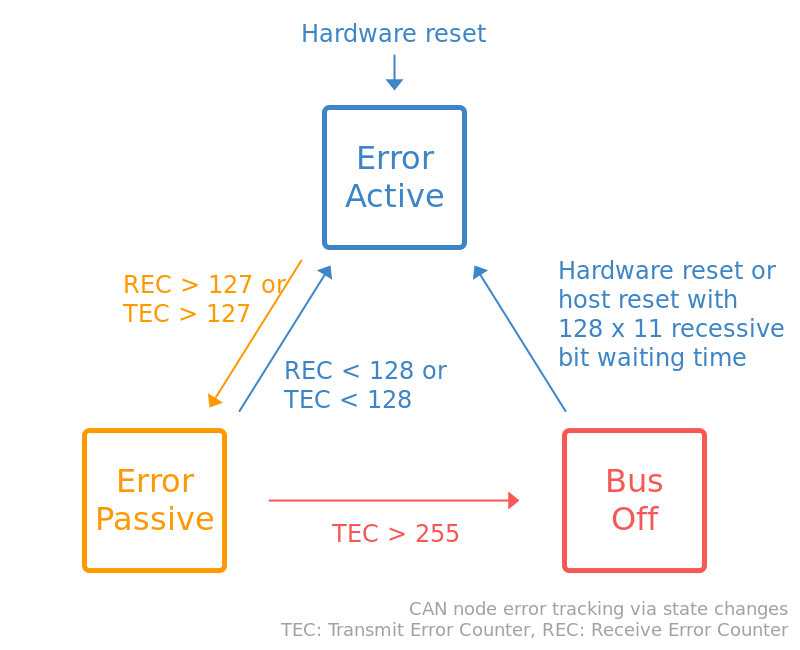
\includegraphics[width=0.6\textwidth]{capitoli/figure-protocolli/CAN-error-states.png}
    \caption{Modalità operative con relative transizioni}
    \label{fig:can-error-states}
\end{figure}

Per tenere traccia della modalità in cui si trova un nodo, vengono impiegati due registri:
\begin{itemize}
    \item \textbf{TEC} (Transmit Error Counter);
    \item \textbf{REC} (Receive Error Counter).
\end{itemize}
L'utilizzo di questi due registri permette ad un nodo di capire come si sta comportando e, in base al valore raggiunto da questi, cambierà modalità e si comporterà come stabilito. I valori dei due registri vengono aggiornati come illustrato nella \autoref{fig:can-error-counter} e, inoltre, nella \autoref{fig:can-error-types} sono illustrati i possibili errori che un nodo può rilevare. \cite{css_electronics_can} \cite{wikipedia_canbus}
\begin{figure}[h]
    \begin{subfigure}{0.45\textwidth}
        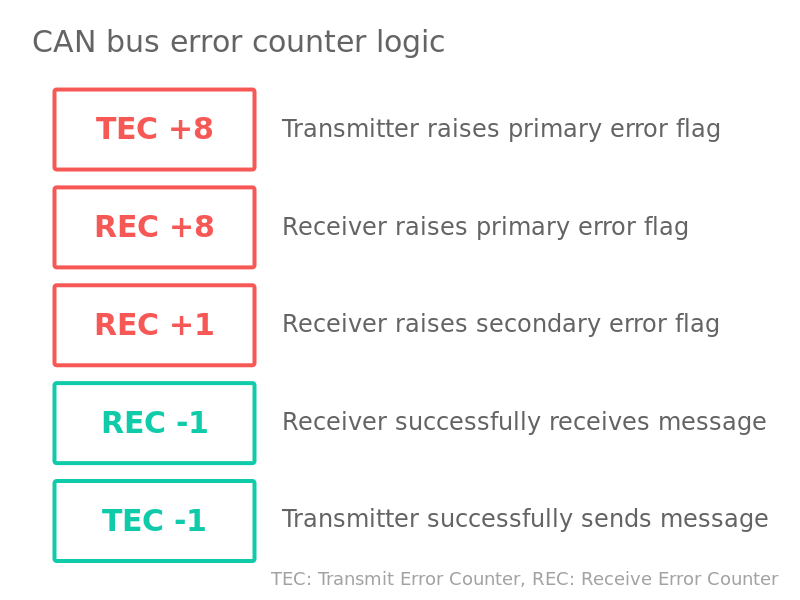
\includegraphics[width=1\textwidth]{capitoli/figure-protocolli/CAN-bus-error-counter.png}
        \caption{Variazioni dei registri di errore}
        \label{fig:can-error-counter}    
    \end{subfigure}
    \hfill
    \begin{subfigure}{0.45\textwidth}
        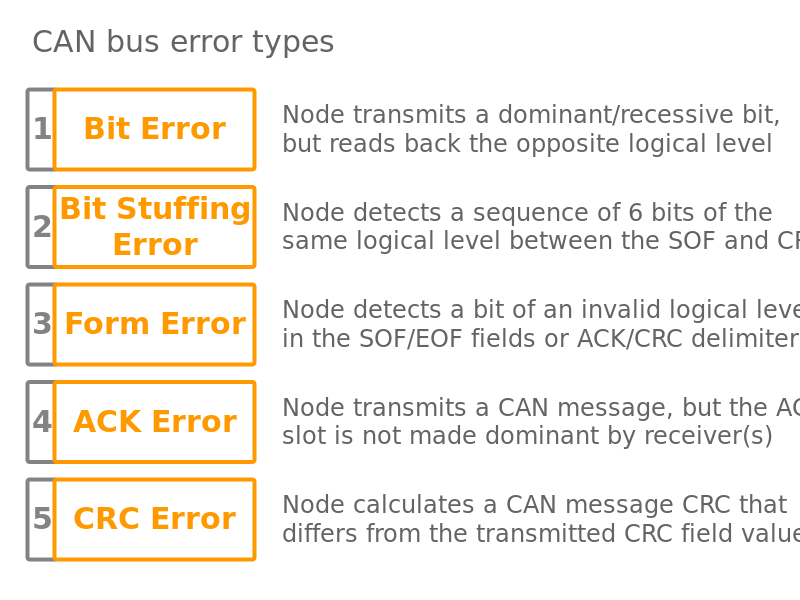
\includegraphics[width=1\textwidth]{capitoli/figure-protocolli/CAN-bus-error-types.png}
        \caption{Errori possibili in \emph{CAN}}
        \label{fig:can-error-types}
    \end{subfigure}
    \caption{Rilevazione e gestione degli errori in \emph{CAN}}
    \label{fig:can-error}
\end{figure}


\subsubsection{Overload Frames}
Questa tipologia di frame permette ad un nodo saturo di avvisare gli altri nodi di fermare la trasmissione di frame di \textbf{dati} e \textbf{remoti}. La struttura è uguale ai frame di \textbf{errore} ma la differenza sta nel momento in cui viene inviato, ovvero durante la trasmissione dell'\textbf{IFS}. \cite{wikipedia_canbus}

\subsection{Varianti del protocollo}
Esistono alcune varianti del protocollo \emph{CAN}, con lo scopo di adattarlo ad ambienti e requisiti diversi. Sebbene se ne possano trovare diverse in letteratura, le principali varianti sono tre.

\subsubsection{Low Speed CAN}
Variante del protocollo con velocità di trasmissione massima di circa 125 Kbps, utilizzata in sistemi con elevati requisiti di affidabilità, che non richiedono una larghezza di banda elevata e che non richiedono aggiornamenti molto frequenti. Il cablaggio richiesto è molto più economico e di solito viene utilizzato in sitemi diagnostici, nei controlli e display del cruscotto, ecc. \cite{can_bus_dewesoft}

\subsubsection{High Speed CAN}
Variante del protocollo con velocità di trasmissione massima di circa 1 Mbps, utilizzata in sistemi che richiedono aggiornamenti molto più frequenti ed un'elevata precisione. Richiede un cablaggio più costoso rispetto alla variante \textbf{Low Speed} ma permette il corretto funzionamento di sistemi \emph{safety-critical} come \textbf{ABS}, airbag, controllo della stabilità, controlli del motore, ecc. \cite{can_bus_dewesoft}

\subsubsection{CAN FD}
Variante del protocollo (chiamata "\emph{CAN} sotto steroidi" \cite{can_bus_dewesoft}) con velocità di trasmissione in grado di raggiungere circa 5 Mbps. Per raggiungere queste velocità si contraddistingue dalle due varianti precedenti sulla lunghezza del payload, dove prima poteva avere una lunghezza massima di 8 Byte mentre con \emph{CAN FD} (Flexible Data-Rate) si possono raggiungere i 64 Byte (incremento dell'800\%). Per realizzare questo incremento, ovviamente, l'header è leggermente diverso da quello standard ma è stato realizzato in modo da essere retrocompatibile con le trasmissioni \emph{CAN} standard.

Le modifiche rispetto ad un frame standard sono:
\begin{itemize}
    \item \textbf{RSS} (Remote Request Substitution) vs \textbf{RTR}: essendo che in \emph{CAN FD} non esistono messaggi \textbf{remoti}, il bit \textbf{RTR} è sostituito con \textbf{RSS} ed è sempre $0$; 
    \item \textbf{FDF} (Flexible Data-Rate Format) vs \textbf{R0}: il bit riservato \textbf{R0} è sostituito con il bit \textbf{FDF} che è sempre $1$ e stabilisce che il messaggio è di tipo \emph{FD}. In questa tipologia di messaggio vengono introdotti anche tre bit aggiuntivi;
    \item \textbf{RES}: 1 bit riservato per sviluppi futuri per cui il suo valore non è influente. È aggiuntivo rispetto al frame standard;
    \item \textbf{BRS} (Bit Rate Switch): 1 bit che se impostato a $0$ indica che la velocità di trasmissione sarà quella della fase di arbitraggio (velocità fino a 1 Mbps) mentre se impostato a $1$ indica che verrà utilizzata una velocità superiore (fino a 5 Mbps). Anche questo è aggiuntivo rispetto al frame standard;
    \item \textbf{ESI} (Error Status Indication): 1 bit che indica la \emph{modalità} in cui è entrato il nodo, quindi sarà $0$ se il nodo è in modalità \textbf{attiva} mentre $0$ se il nodo è in modalità \textbf{passiva}. Anche questo nodo è aggiuntivo rispetto al frame standard;
    \item \textbf{DLC}: Come nei frame standard, anche qui indica la lunghezza del payload. Tuttavia, a differenza dello standard, la corrispondenza tra valore in bit e lunghezza è leggermente diversa per permettere l'invio di payload più lunghi di 8 byte (la mappatura è indicata in \autoref{fig:canfd-dlc});
    \item \textbf{SBC} (Stuff Bit Count): 3 bit che rispettano la codifica di Gray, seguiti da un bit di parità. Sono stati aggiunti per migliorare l'affidabilità della comunicazione;
    \item \textbf{CRC}: 17 bit o 21 bit per il controllo degli errori dei payload di 16 Byte o 20-64 Byte, rispettivamente. A differenza dei messaggi standard, nei messaggi \emph{CAN FD} sono impostati \textbf{SEMPRE} 4 bit di stuffing, mentre prima potevano essercene tra 0 e 3;
    \item \textbf{FSB} (Fixed Stuff Bit): bit di stuffing impostati prima e dopo \textbf{SBC} e all'interno del campo \textbf{CRC};
    \item \textbf{ACK}: questo campo delimita la fine dell'invio a velocità superiori, ritornando alla velocità di default di \emph{CAN}.
\end{itemize}

\begin{figure}[h]
    \begin{subfigure}{0.45\textwidth}
        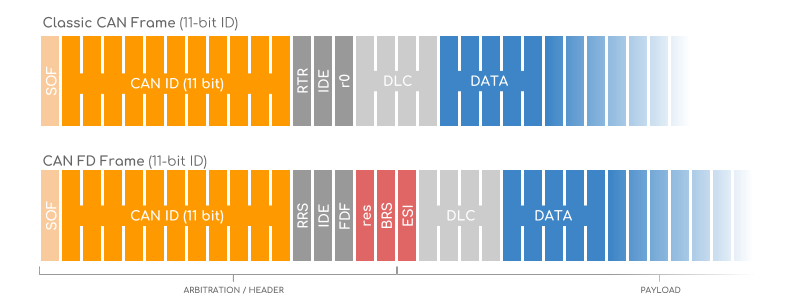
\includegraphics[width=1\textwidth]{capitoli/figure-protocolli/canfd-header.png}
        \caption{Header \emph{CAN FD} vs. header \emph{CAN}}
        \label{fig:canfd-header}
    \end{subfigure}
    \hfill
    \begin{subfigure}{0.45\textwidth}
        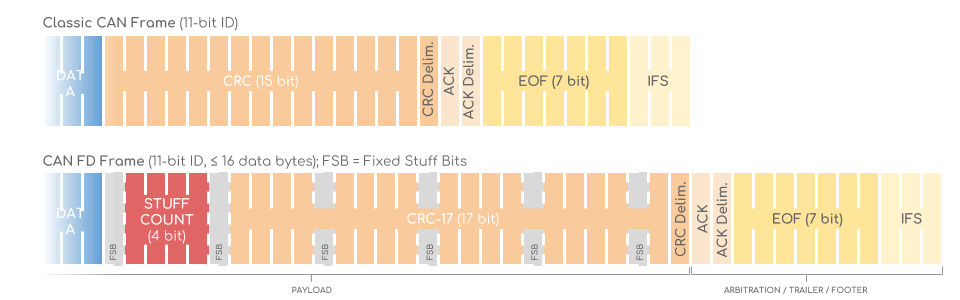
\includegraphics[width=1\textwidth]{capitoli/figure-protocolli/canfd-trailer.png}
        \caption{Trailer \emph{CAN FD} vs. trailer \emph{CAN}}
        \label{fig:canfd-trailer}
    \end{subfigure}
    \centering
    \begin{subfigure}{0.8\textwidth}
        \vspace{0.3cm}
        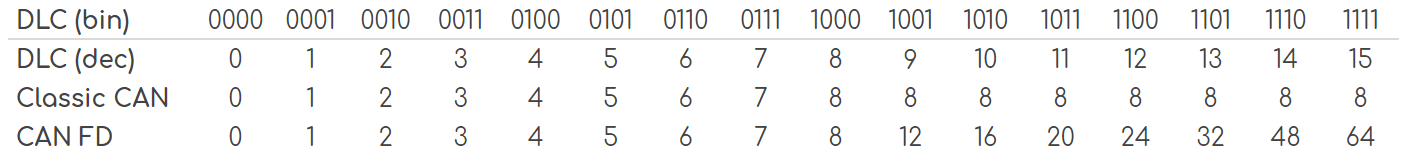
\includegraphics[width=1\textwidth]{capitoli/figure-protocolli/canfd-dlc.png}
        \caption{Mappatura dei valori di \textbf{DLC} in \emph{CAN FD} e \emph{CAN}}
        \label{fig:canfd-dlc}
    \end{subfigure}
    \caption{Differenze tra \emph{CAN FD} e \emph{CAN}}
    \label{fig:canfd-differences}
\end{figure}

Un altro vantaggio molto importante che introduce questa variante è la possibilità di variare in maniera adattiva la velocità di trasmissione dei messaggi. Questo permette ai nodi di adattarla in base a ciò che si vuole inviare, lasciando la velocità invariata o accelerando in caso di dati più urgenti o messaggi più lunghi.

Rispetto alla variante standard, con \emph{CAN FD} si possono realizzare sistemi più complessi che richiedono requisiti di banda più stringenti. Ad esempio, si possono realizzare sistemi \textbf{ADAS} (Advanced Driver Assistance System) come cruise control adattivo, frenata automatica d'emergenza, moonitoraggio degli angoli ciechi, ecc. \cite{css_electronics_canfd}

\section{FlexRay}

\section{LIN}

\section{Confronto tra i tre protocolli}

\newpage
